\section{NumPy}
\subsection{Einführung}
NumPy (Numerical Python) ist eine Bibliothek zur Durchführung mathematischer Funktionen und Operationen auf großen mehrdimensionalen Arrays. Sie bietet:
\begin{itemize}
    \item \textbf{Geschwindigkeit}: Verwendet optimierten C-Code und ersetzt langsame Standard-Python \texttt{for}-Schleifen.
    \item \textbf{Vektorisierung}: Arraybasierte Operationen werden automatisch elementweise ausgeführt.
    \item \textbf{Broadcasting}: Erweitert implizit Arrays unterschiedlicher Formate während arithmetischen Berechnungen.
\end{itemize}

\subsection{Erstellung von n-dimensionalen Arrays (\texttt{ndarray})}
Das \texttt{ndarray} ist eine homogene Datenstruktur, in der jede Dimension als \textit{Achse} bezeichnet wird.
\begin{itemize}
    \item \texttt{arr.ndim}: Anzahl der Dimensionen.
    \item \texttt{arr.shape}: Tupel, das die Größe jeder Dimension darstellt. (rows, cols)
    \item \texttt{arr.dtype}: Datentyp der Array-Elemente (z.B. \texttt{np.float64}, \texttt{np.int32}).
    \item \texttt{arr.astype(dtype)}: Gibt eine Kopie des Arrays zurück, die in einen bestimmten Typ umgewandelt wurde.
\end{itemize}

\subsubsection{Array-Erstellungsmethoden}
\lstinputlisting[language=Python]{code/np_array_creation.py}


\resizebox{\columnwidth}{!}{
\begin{tabular}{l|l}
\textbf{Funktion} & \textbf{Resultat} \\ \hline
\texttt{np.ones((2,2))} & \texttt{array([[1., 1.], [1., 1.]])} \\
\texttt{np.ones\_like(arr1)} & \texttt{array([1, 1, 1])} \\
\texttt{np.zeros((2,2))} & \texttt{array([[0., 0.], [0., 0.]])} \\
\texttt{np.zeros\_like(arr1)} & \texttt{array([0, 0, 0])} \\
\texttt{np.full((2,2), 7.0)} & \texttt{array([[7., 7.], [7., 7.]])} \\
\texttt{np.full\_like(arr1, 7)} & \texttt{array([7, 7, 7])} \\
\texttt{np.eye(2)} & \texttt{array([[1., 0.], [0., 1.]])} \\
\texttt{np.linspace(0, 1, 5)} & \texttt{array([0., 0.25, 0.5, 0.75, 1.])} \\
\texttt{np.arange(0, 4, 0.5)} & \texttt{array([0, 0.5, 1, 1.5, 2, 2.5, 3, 3.5])} \\
\texttt{np.logspace(0, 1, 4)} & \texttt{array([1., 2.1544, 4.6416, 10.])} \\
\texttt{np.random.randn(3)} & \texttt{array([0.7576, 0.0135, -0.8934])} \\
\texttt{np.random.randint(0,10,3)} & \texttt{array([0, 5, 4])} \\
\end{tabular}}\medbreak

Bei \texttt{arange} ist es möglich, einen negativen \texttt{step} anzugeben, um ein absteigendes Array zu erzeugen.

\crd{Achten Sie darauf, dass \texttt{end} aus dem Array ausgeschlossen ist,} wenn Sie einschließen möchten: (\texttt{end} $\pm$ \texttt{step})

\columnbreak

\subsection{Elementzugriff}
\begin{itemize}
    \item \textbf{Indexing}: Achsen werden durch Kommas innerhalb von eckigen Klammern getrennt (z.B. \texttt{arr[row, col]}).
    \item \textbf{Slicing}: Folgt der \texttt{[start:end:step]}-Syntax über mehrere
     Achsen hinweg. Slicing gibt eine \textbf{view} zurück; Änderungen wirken sich auf das ursprüngliche Array aus. 
     Verwenden Sie \texttt{.copy()}, um eine unabhängige Duplikatkopie zu erstellen.
     \crd{END not included!}
    \item \textbf{Boolean Slicing}: Extrahiert Teilmengen, bei denen eine Bedingung \texttt{True} ist (z.B. \texttt{arr[arr > 5]}).
    \item \textbf{Unpacking}: Eine Matrix kann direkt in ihre Bestandteile entlang 
    der ersten Achse entpackt werden: \lstinline[language=Python]|row1, row2 = np_matrix|
\end{itemize}

\textbf{Beispiele:}

\begin{center}
    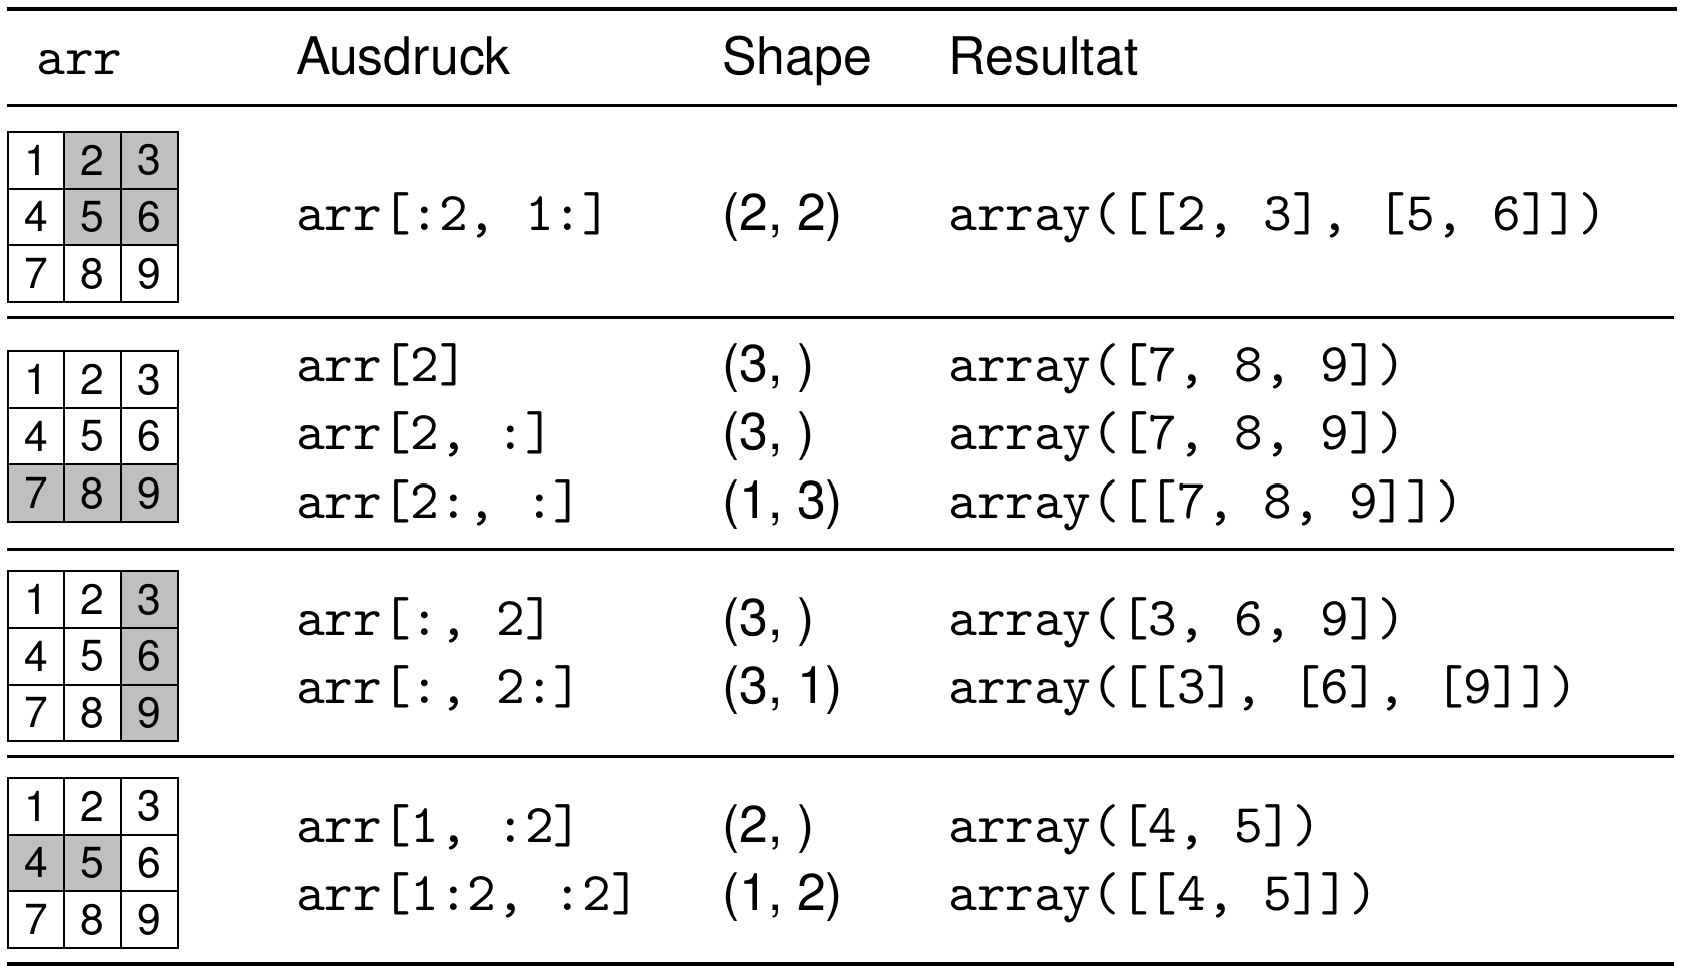
\includegraphics[width=0.7\linewidth]{images/slicing.png}
\end{center}

\begin{minipage}{0.45\columnwidth}
    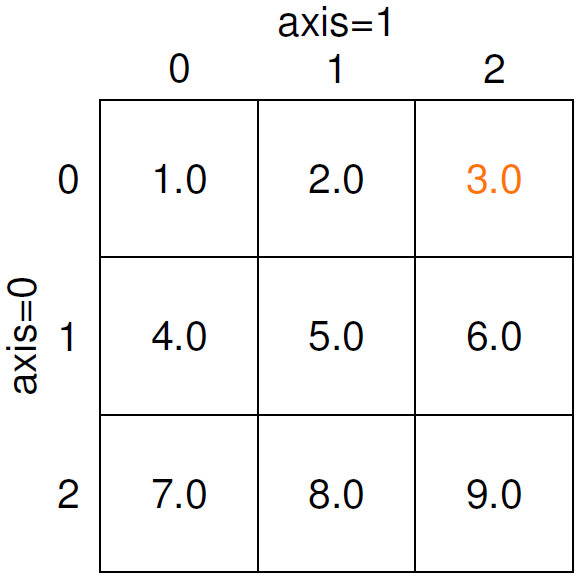
\includegraphics[width=\linewidth]{images/indizierung3.png}
\end{minipage}\hfill
\begin{minipage}{0.45\columnwidth}
    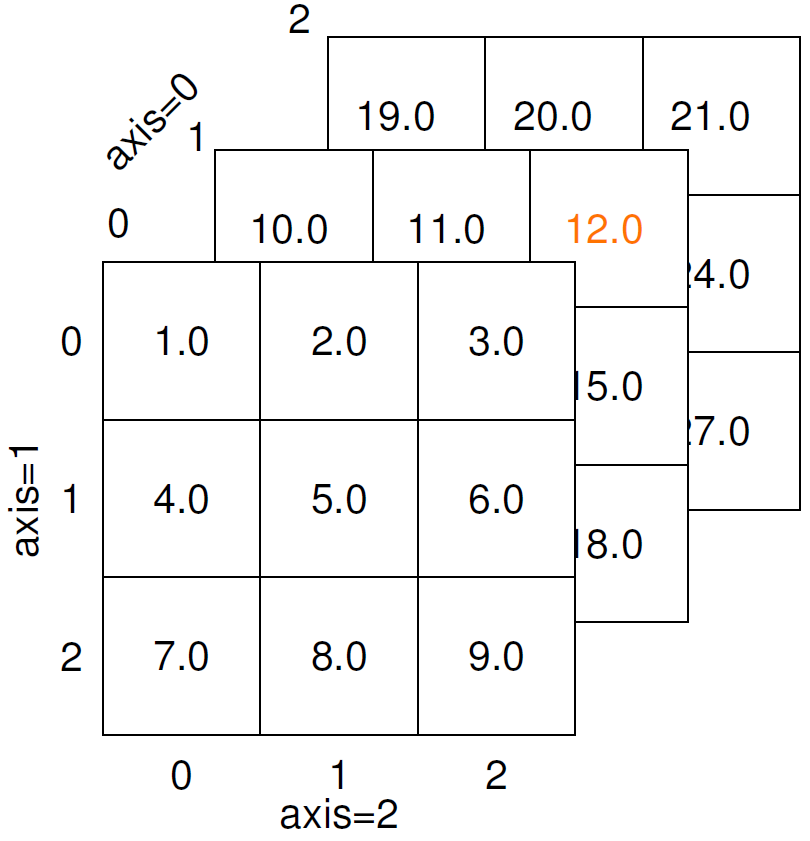
\includegraphics[width=\linewidth]{images/indizierung4.png}
\end{minipage}

Die Achsen ändern sich immer, wenn Dimensionen hinzugefügt/entfernt werden

\subsection{Broadcasting}
Um Operationen auf Arrays unterschiedlicher Formen auszuführen, broadcastet NumPy automatisch das kleinere Array:
\begin{enumerate}
    \item Dimensionen werden links eingefügt, bis die Anzahl der Dimensionen (\texttt{ndim}) übereinstimmt.
    \item Dimensionen der Größe 1 werden gestreckt, um der entsprechenden Dimension des anderen Arrays zu entsprechen.
    \item Wenn die Größen unterschiedlich sind und weder das eine noch das andere 1 ist, wird ein \texttt{ValueError} ausgelöst.
\end{enumerate}

\subsection{Array-Manipulation}
\subsubsection{Verkettung und Stacking}
\lstinputlisting[language=Python]{code/np_concatenation.py}


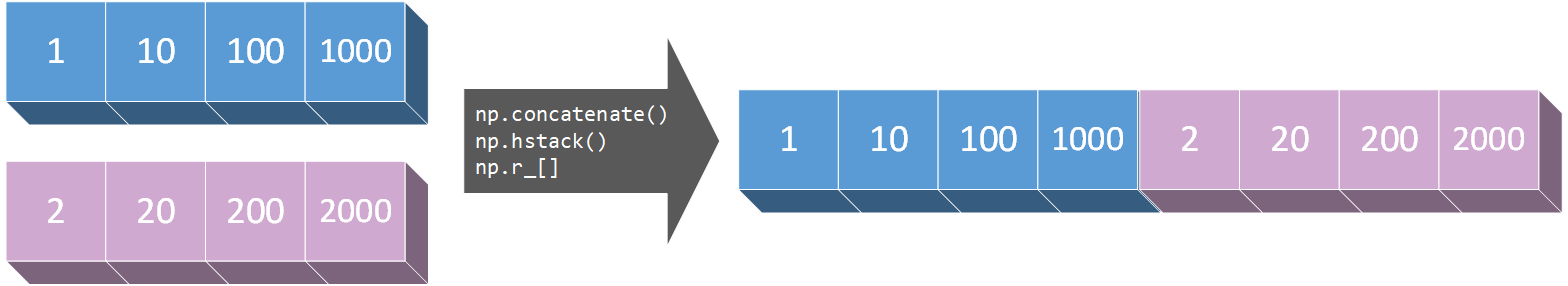
\includegraphics[width=\linewidth]{images/stacking_1D_1D.png}
\begin{center}
    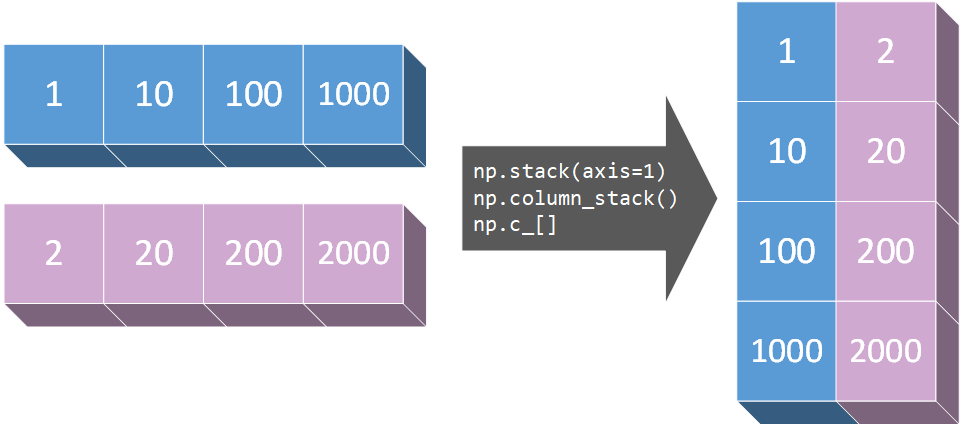
\includegraphics[width=0.7\linewidth]{images/stacking_1D_2D_spaltenweise.png}
\end{center}

\subsubsection{Dimensionsänderungen}
\lstinputlisting[language=Python]{code/np_dimesnions.py}

\begin{itemize}
    \item \textbf{View vs Copy}: \texttt{arr.reshape(-1)} erzeugt eine \textbf{view} und keine physische Kopie. Das Ändern des umgeformten Arrays wirkt sich auf das ursprüngliche aus.
    \item \textbf{Automatic Reshaping}: Die Verwendung von \texttt{-1} ermöglicht es NumPy,
    eine Dimension automatisch anhand der gesamten Größe des Arrays zu berechnen.
    \item \textbf{Kompatibilitätsbedingung}: Es kann nur eine Dimension auf \texttt{-1} gesetzt werden.
    Damit ein reshape gültig ist, muss die gesamte Anzahl der Elemente $N$ 
    genau durch das Produkt der angegebenen Dimensionen teilbar sein.
\end{itemize}


\subsection{Mathematische Funktionen}
NumPy stellt vektorisierte universelle Funktionen (ufuncs) wie \texttt{np.exp()}, \texttt{np.sin()}, \texttt{np.abs()}, \texttt{np.mean()}, \texttt{np.max()}, \texttt{np.std()} und \texttt{np.cumsum()} bereit.

% --- SUBSECTION: ADVANCED CONCATENATION & LINEAR ALGEBRA ---
\subsection{Verkettung}
\textbf{MATLAB-like Concatenation:}

\begin{itemize}
    \item \texttt{np.r\_}: Verkettet entlang der ersten Achse (zeilenweise). Es unterstützt Slice-Objekte und einzelne Werte.
    \item \textit{Beispiel:} \texttt{x = np.r\_[1:5, 15, 20:50:10]} $\rightarrow$ \texttt{[1, 2, 3, 4, 15, 20, 30, 40]}
    \item \texttt{np.c\_}: Verkettet entlang der zweiten Achse (spaltenweise). Ideal zum Erstellen von Spaltenvektoren.
    \item \textit{Beispiel:} \texttt{y = np.c\_[0:3]} $\rightarrow$ \texttt{[[0], [1], [2]]}
\end{itemize}

\subsection{NumPy Lineare Algebra: Multiplikation Zusammenfassung}

\subsubsection{Skalar- und Vektorprodukte}
\begin{itemize}
    \item \textbf{np.inner(a, b):} Am besten für das \textbf{Skalarprodukt} (inner product) zweier Vektoren. 
    \begin{itemize}
        \item \textit{Wann verwenden:} Verwenden Sie es, wenn Sie explizit das Skalarprodukt von Vektoren möchten. Es ist klarer als \texttt{dot()}, weil es auf diese spezifische Operation beschränkt ist.
        \item \textit{Beispiel:} \texttt{v1 = [1, 2]; v2 = [3, 4] $\to$ 1*3 + 2*4 = 11}.
    \end{itemize}
    
    \item \textbf{np.outer(a, b):} Berechnet das \textbf{dyadische Produkt} (outer product).
    \begin{itemize}
        \item \textit{Wann verwenden:} Verwenden Sie es, um eine Matrix aus zwei Vektoren zu erzeugen (Spaltenvektor $\times$ Zeilenvektor).
        \item \textit{Beispiel:} \texttt{v1 = [1, 2]; v2 = [3, 4] $\to$ [[3, 4], [6, 8]]}.
    \end{itemize}
\end{itemize}

\subsubsection{Matrixmultiplikation: @ vs np.dot()}
Während beide die standardmäßige Matrixmultiplikation für 2D-Arrays ausführen, verhalten sie sich für höherdimensionale Tensoren ($n > 2$) unterschiedlich.

\begin{itemize}
    \item \textbf{Der @-Operator (np.matmul):} Der Standard für \textbf{Matrixmultiplikation}.
    \begin{itemize}
        \item \textit{Verhalten ($n > 2$):} Er behandelt das Array als eine 'stack' von Matrizen und multipliziert sie über ihre letzten zwei Dimensionen hinweg.
        \item \textit{Empfehlung:} Dies ist die bevorzugte Methode für die standardmäßige Matrixmultiplikation in modernem Python (3.5+).
    \end{itemize}
    
    \item \textbf{np.dot(a, b):}
    \begin{itemize}
        \item \textit{Verhalten ($n > 2$):} Es berechnet die Summe der Produkte über der \textbf{letzten} Dimension von $a$ und der \textbf{vorletzten} Dimension von $b$.
        \item \textit{Ergebnis:} Es multipliziert effektiv die erste Zeile von $a$ mit JEDER Spalte in jeder nachfolgenden Matrix von $b$, was zu einer deutlich größeren resultierenden Form führt.
    \end{itemize}
\end{itemize}

\cor{Meistens immer den \texttt{@}-Operator verwenden}
\subsubsection{Vergleichsbeispiel ($n > 2$)}
\lstinputlisting[language=Python]{code/comparison_dot.py}

\subsubsection{Methoden}
Das Modul \texttt{np.linalg} stellt essentielle Werkzeuge für Matrixberechnungen bereit.

\begin{itemize}
    \item \textbf{np.linalg.solve(A, b)}: Berechnet die exakte Lösung einer linearen Matrixgleichung $Ax = b$.
    \begin{itemize}
        \item  $A$ muss quadratisch und von vollem Rang (nicht singulär) sein.
    \end{itemize}

    \item \textbf{np.linalg.lstsq(A, b, rcond=None)}: Gibt die \textbf{Least-Squares}-Lösung zu einer linearen Matrixgleichung zurück.
    \begin{itemize}
        \item \textit{Wann verwenden}: Wenn $Ax = b$ keine exakte Lösung hat 
        \item \textit{Gibt Array zurück}: Ein Tupel, das die Lösung $x$, die Residuen, den Rang von $A$ und die singulären Werte enthält.
    \end{itemize}

    \item \textbf{np.linalg.eig(A)}: Berechnet die Eigenwerte und die rechten Eigenvektoren eines quadratischen Arrays.
    \begin{itemize}
        \item \textit{Rückgabe}: Ein Tupel \texttt{(w, v)}, wobei \texttt{w} die 
        Eigenwerte enthält und \texttt{v} die entsprechende Matrix mit Eigenvektoren als Spalten.
    \end{itemize}
    \item \texttt{np.linalg.inv(A)}: Berechnet die multiplikative Inverse einer quadratischen Matrix.
    \item \texttt{np.linalg.det(A)}: Berechnet die Determinante einer Matrix.
    \item \texttt{np.trace(A)}: Berechnet die Spur, d.h. die Summe der Diagonalelemente eines Arrays .
    \item \texttt{np.linalg.matrix\_rank(A)}: Gibt den Rang der Matrix eines Arrays zurück.
    \item \texttt{np.linalg.norm(R)}: Berechnet die euklidische Norm (Betrag), definiert als die Quadratwurzel aus der Summe der Quadrate der Komponenten des Vektors  Formel: $||p||_{2} = \sqrt{x^{2} + y^{2} + z^{2}}$.
\end{itemize}

\textbf{Beispielverwendung:}
\lstinputlisting[language=Python]{code/linalg_methods_example.py}

\section{Datenvorverarbeitung und -bereinigung}

\subsection{Resampling}
\lstinputlisting[language=Python]{code/resampling.py}


\subsection{Datenbereinigung \& Skalierung}
\lstinputlisting[language=Python]{code/data_cleaning.py}

\subsection{NumPy Dateiverwaltung}
\lstinputlisting[language=Python]{code/np_file_handling.py}